\section{Background}\label{sec:background}

\subsection{Accumulation and inherited state}\label{sec:decay}

Lehman's laws and Parnas's software-aging account motivate maintenance
alongside growth~\cite{lehman1980laws,lehman1997metrics,parnas1994aging}.
The 1997 formulation states the declining-quality law; it supplies no
data for or against it. Eick et~al. report mixed evidence from
fifteen-plus years of change history~\cite{eick2001decay}, and a systematic
review finds uneven support across systems~\cite{herraiz2013laws}.
Neither feature count nor churn is itself decay. A regression loses
still-required, previously working behaviour; an unimplemented capability
is an acquisition failure. Repeated failure is persistence, not proof
that an earlier defect caused a distinct later one.

Cunningham describes shipping first-time code and rewriting it as
understanding improves~\cite{cunningham1992wycash}. Fowler's design
stamina is explicitly a hypothesis~\cite{fowler2007stamina}.
Reported debt costs concern different settings: a vendor-associated
39-codebase study reports 124\% longer issue resolution in low-quality
files~\cite{tornhill2022codered}; 43 developers self-report about 23\%
of working time lost to debt~\cite{besker2018cripples}.
These are not universal productivity coefficients.

\paragraph{What survives the next session?}\label{sec:inheritance}
Code, tests and deployment assumptions survive through the repository;
instructions and handovers survive through procedural context.
Either channel can preserve a sound decision or a mistake.
Here ``software entropy'' is an engineering analogy, not a
thermodynamic measure. The proposed outcomes are retained behaviour,
adaptation and resource use.

\begin{figure}[!htbp]
\centering
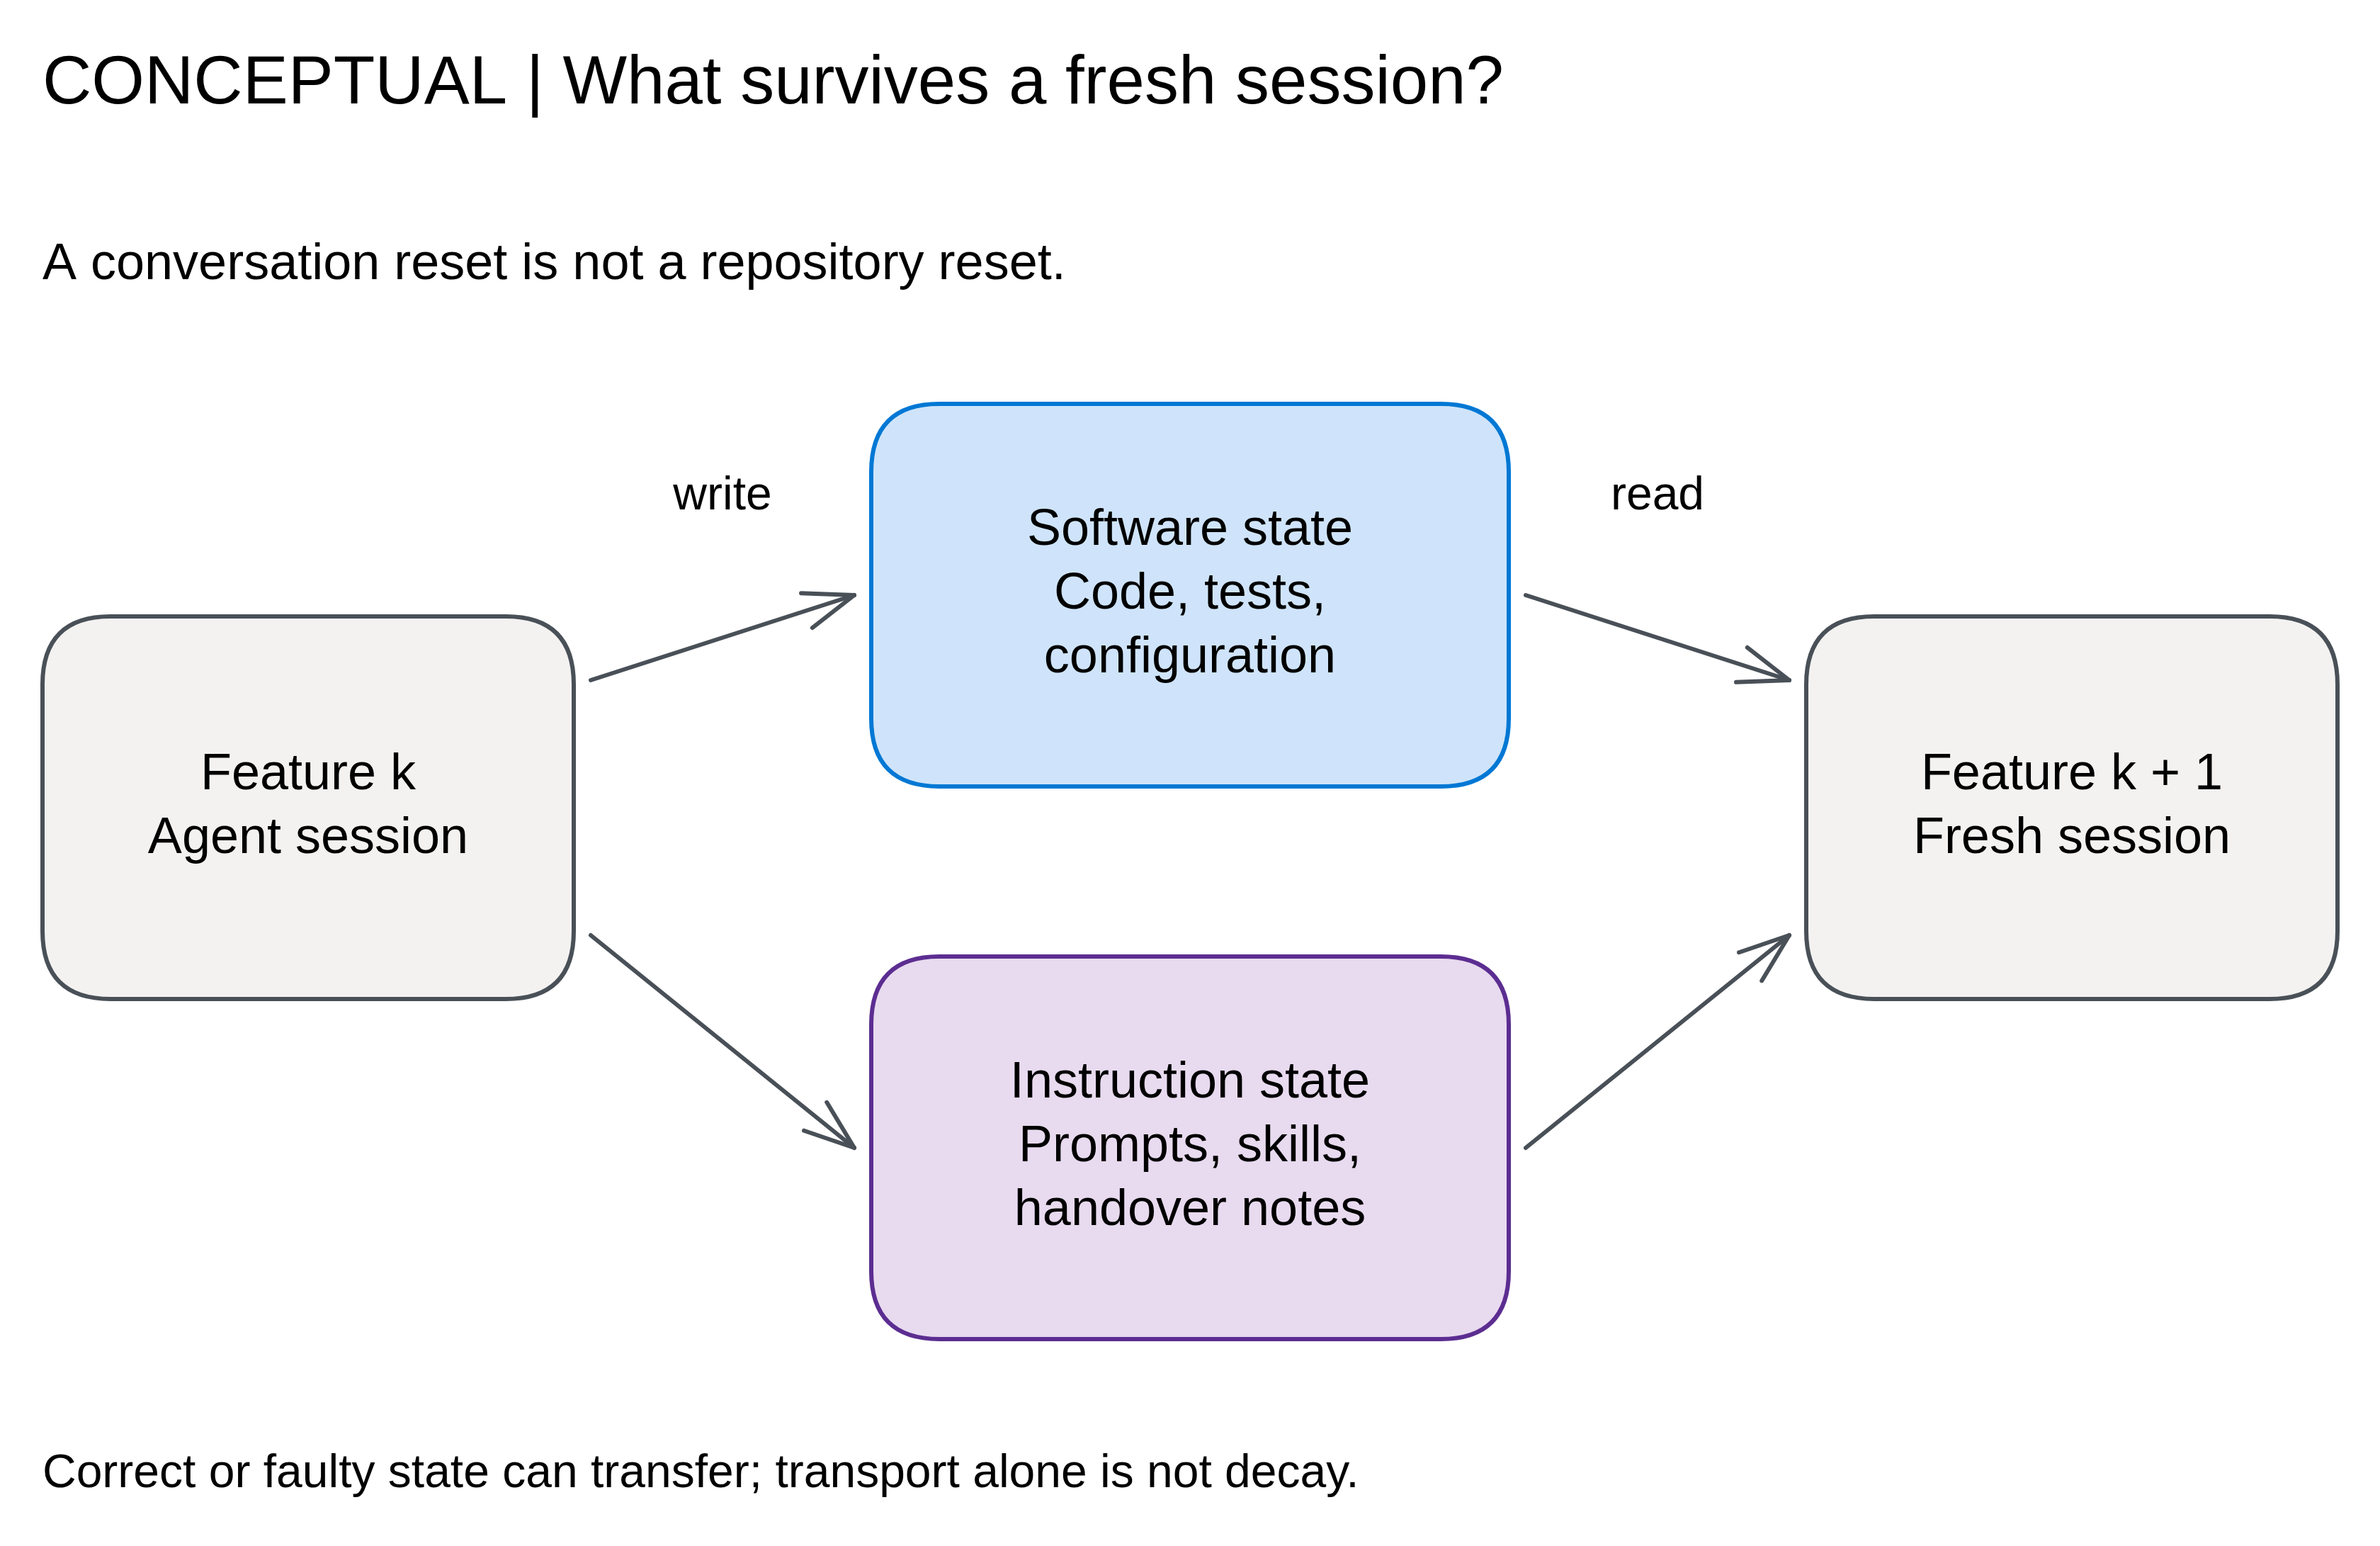
\includegraphics[width=\linewidth]{fig-state-inheritance.png}
\caption{Conceptual read/write paths between sessions. A fresh conversation
does not reset software or instructions. Arrows are possible state transfer,
not measured error propagation.}\label{fig:stateinheritance}
\end{figure}

\subsection{Evidence within and between features}\label{sec:empirical}

Conversational benchmarks identify dependence on erroneous histories,
not merely context length. Zhang et~al. study false justifications after
wrong answers~\cite{zhang2023snowball}; Sinha et~al. vary erroneous prior
state updates in a controlled execution task
~\cite[Secs.~2.2--3, Figs.~5--6]{sinha2025illusion}.
Laban et~al.'s 39\% relative multi-turn performance drop concerns
simulated underspecified conversations, not repository defects;
locators refer to their arXiv v1
~\cite[Secs.~3.3, 6.1, App.~F]{laban2025lost}.

Pan et~al.'s SWE-Maintain more directly tests repository inheritance:
100 three-event episodes from 50 Python repositories, with fresh
sessions and matched later tasks under developer and agent histories.
Across 1,996 paired later events, agent history reduces current-task
resolution by 5.6 points; requiring earlier tests also to pass gives
a 14.0-point gap. Unweighted mean current-task gaps grow from 4.0 to
7.2 points between the second and third events. In the selected
619-event clean-history subset, the current-task difference is
$-1.1$ points, interval $[-3.8,+1.6]$, and cumulative event resolution
differs by $+2.7$, interval $[-0.5,+6.1]$
~\cite[Secs.~4.1--4.2, Tables~2--3]{pan2026swemaintain}.
This favours inherited behavioural failures over complexity alone as
the main observed channel, without establishing a general decay law
or a randomised repair effect.

\begin{figure}[!htbp]
\centering
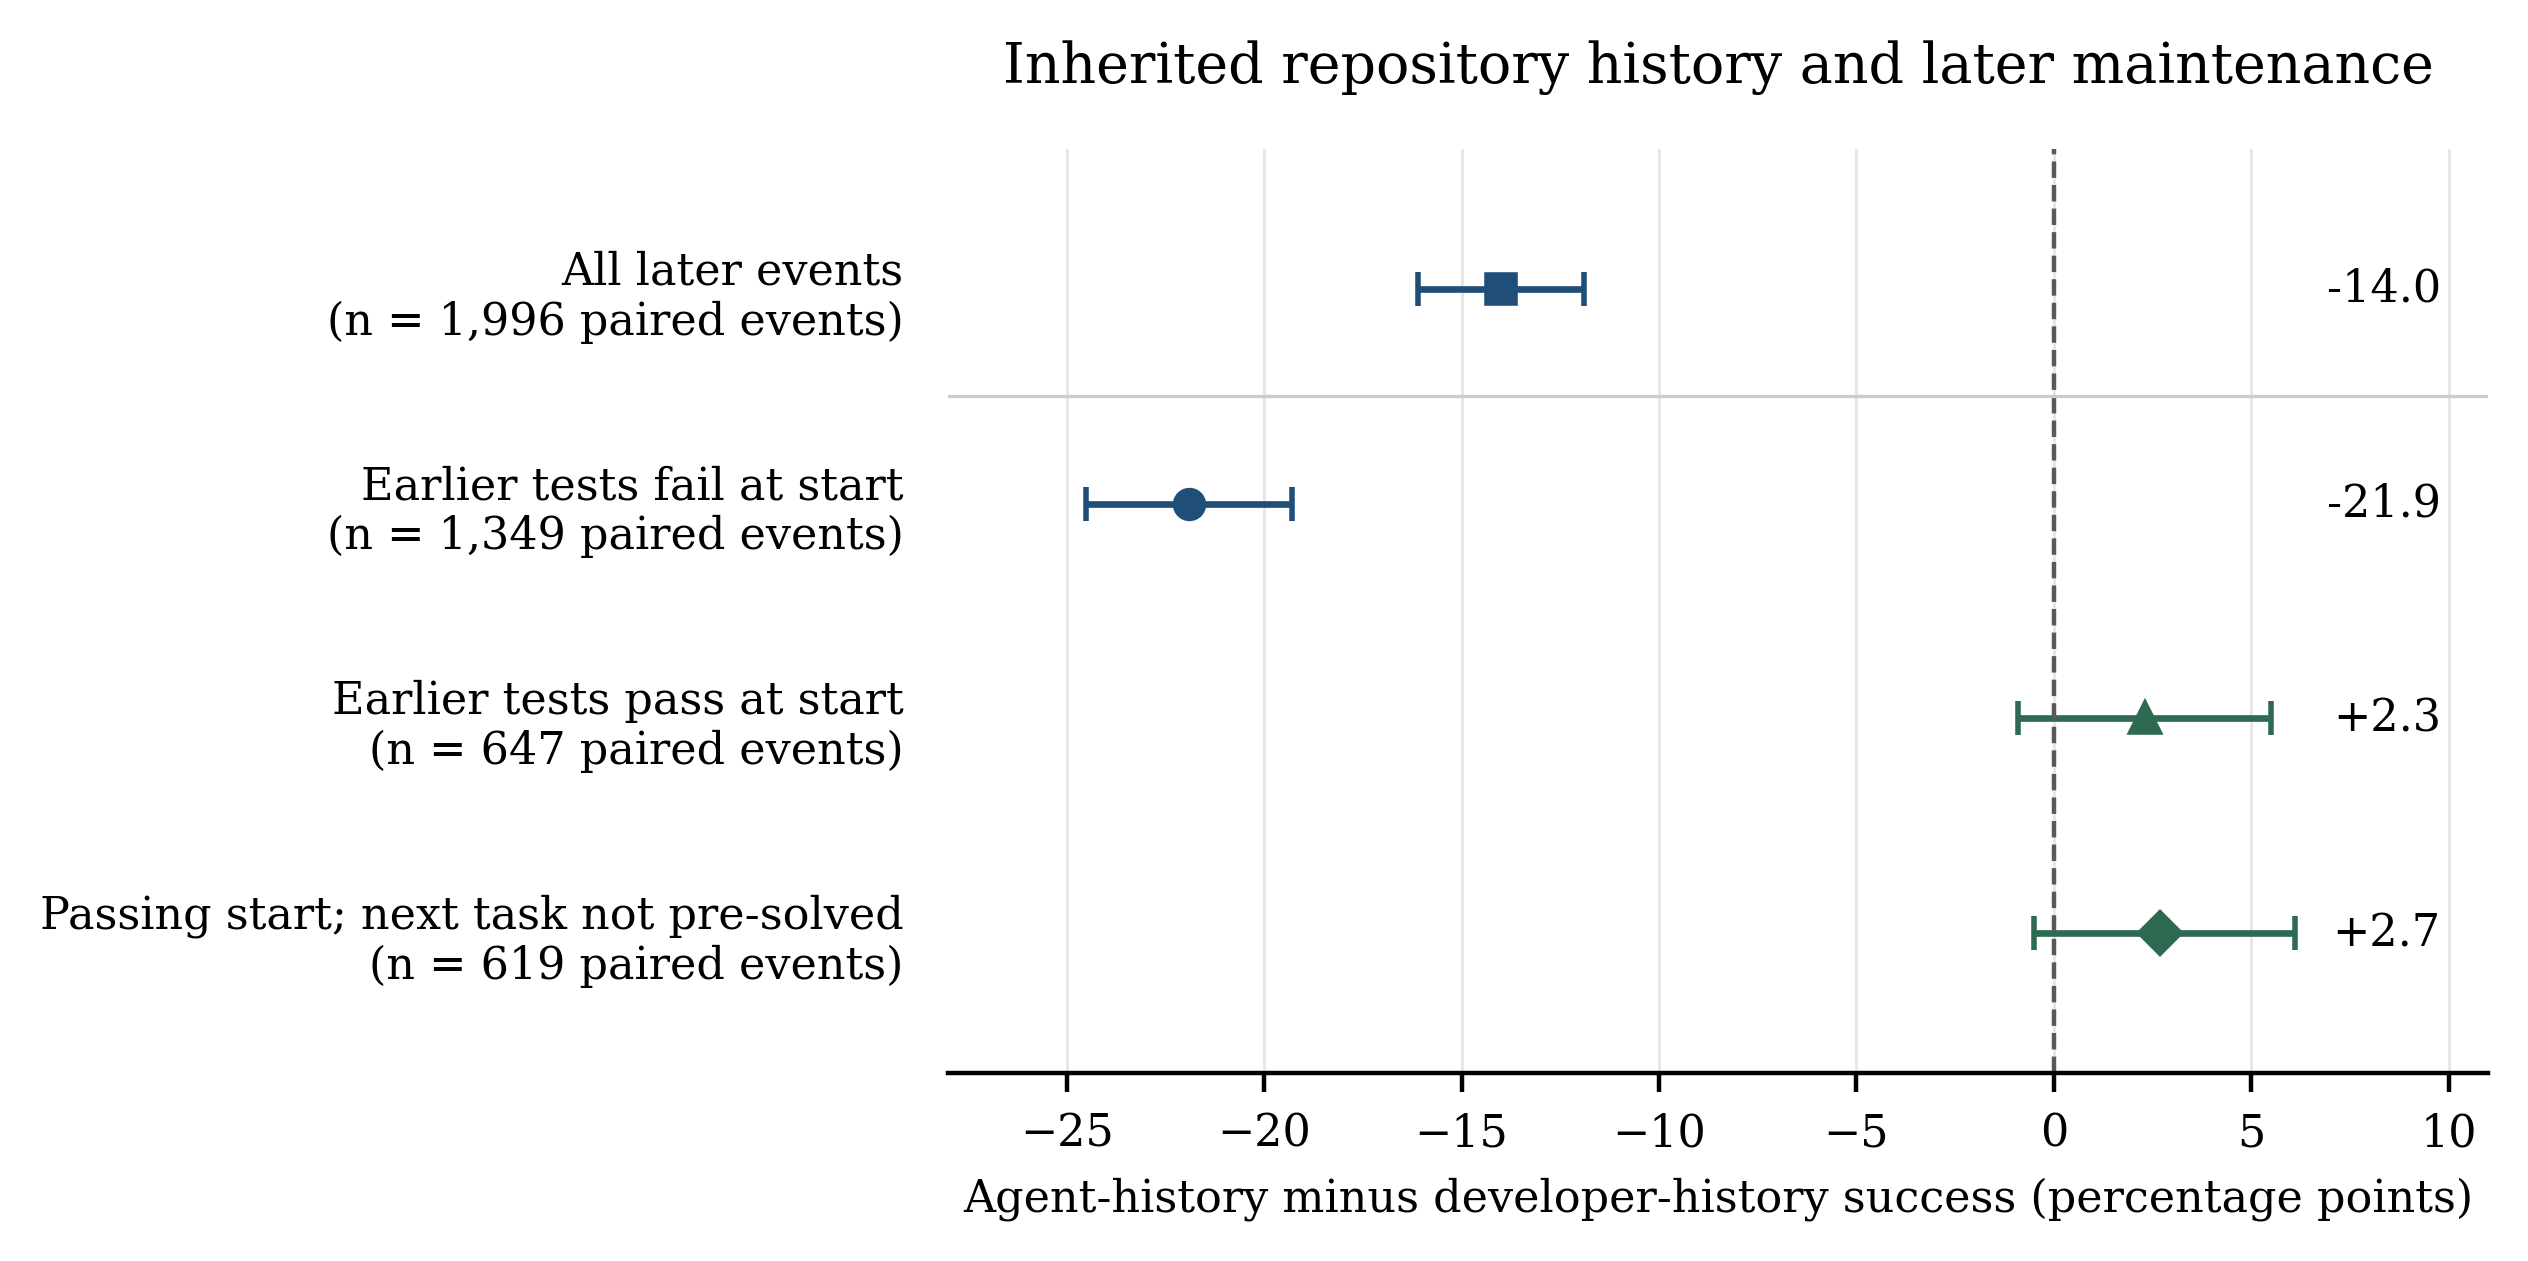
\includegraphics[width=\linewidth]{fig-inherited-history.png}
\caption{Published event-resolution differences and repository-clustered
95\% intervals from Pan et~al., Table~3. Current and prior
non-superseded tests must pass. Selected cohorts overlap; they are
not independent studies or randomised repair conditions.
Values and whiskers are transcribed, not fitted here.}
\label{fig:inheritedhistory}
\end{figure}

Their \texttt{python\_unidiff} example reuses line-splitting logic that
loses terminators in a later constructor; Figure~1's caption introduces
it and Section~5.1/Figure~5 supplies the detail
~\cite{pan2026swemaintain}. SlopCodeBench and SWE-CI extend iterative
evaluation~\cite{orlanski2026slopcodebench,chen2026sweci}.
Borg et~al.'s maintainability study finds no significant downstream
difference for late-2024 assistants; only phase two was randomised
~\cite{borg2025echoes}. This is a counterexample, not a test of the
current autonomous roster.

\subsection{Instruction maintenance and evaluation}\label{sec:instructiondebt}

Instructions are maintained artifacts, not automatically reliable
memory~\cite{nigh2025agentsmd,rajasekaran2025context}.
Mohsenimofidi et~al.'s 169 commits have 242 overlapping assignments
across nine categories; 78 instruction additions, 59 modifications
and 23 removals are three categories, not a partition
~\cite[Sec.~4.3, Table~2]{mohsenimofidi2026context}.
Chatlatanagulchai et~al.'s sampled maintenance labels likewise include
addition and pruning~\cite{chatlatanagulchai2026readmes}.
Instruction debt here is the author's term for obsolete, duplicated,
conflicting or poorly routed directives.

\begin{figure}[!htbp]
\centering
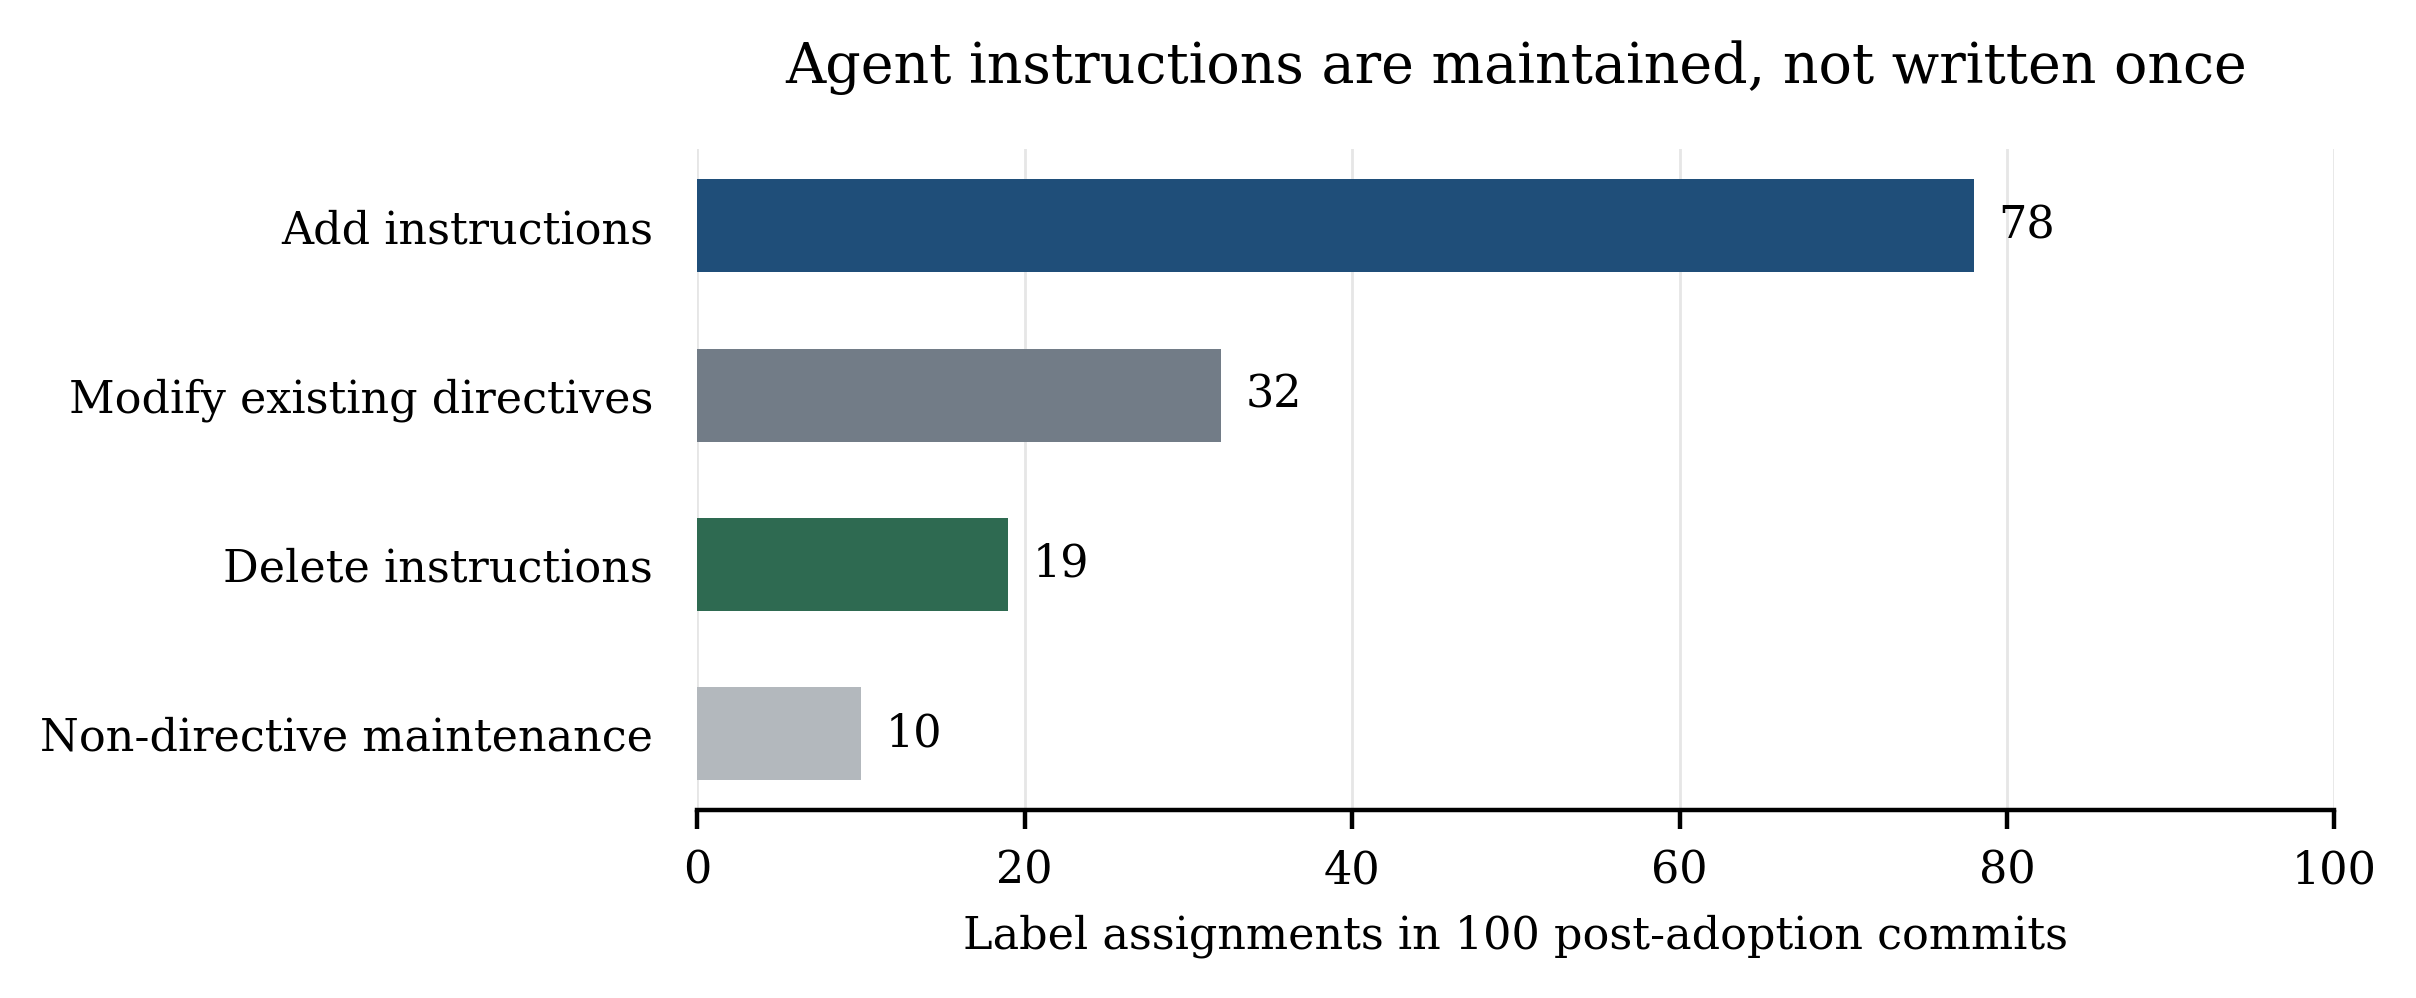
\includegraphics[width=0.94\linewidth]{fig-instruction-maintenance.png}
\caption{Labels in 100 sampled post-adoption commits, from
Chatlatanagulchai et~al., Sections~4.2.2--4.2.3. Labels overlap and
count edit types, not net token growth or effects on agent success.}
\label{fig:instructionmaintenance}
\end{figure}

Gloaguen et~al. report 20\%/23\% higher inference cost with LLM-written
context and slightly lower success, by 0.5/2 points, without significant
differences from no-file baselines. Developer-written files outperform
LLM-written ones on CTXbench ($p=0.038$)
~\cite[Sec.~4.2, Tables~2--3]{gloaguen2026agentsmd}.
SkillOpt and Jiang et~al. provide counterevidence to treating retained
instructions as inherently harmful: evaluated procedural guidance can
help, while retrieval and downstream success remain distinct
~\cite{microsoft2026skillopt,jiang2026skills}.

\paragraph{Tests and review.}\label{sec:evaluationwork}
RefactorBench studies refactoring, not between-feature consolidation
~\cite{gautam2025refactorbench}; developer-agent collaboration studies
are observational~\cite{kumar2025agents}.
SWE-Sharp-Bench supplies reproducible repository evaluation
~\cite{mhatre2025swesharp}, while CRBugBench exposes review limits
~\cite{yang2026crbugbench}. Building to the Test finds a dead or
absent required library in seven of twelve oracle-in-the-loop runs
~\cite{ma2026building}. ImpossibleBench tests exploitation more broadly
~\cite{zhong2026impossiblebench}. Test integrity and adequate outcome
coverage are different requirements. AgentRx motivates traceable
failure diagnosis~\cite{microsoft2026agentrx}.

\paragraph{Bounded correction.}\label{sec:factory}
Pavlenko et~al.'s factory optimises human-architected systems against
measurable objectives; productivity estimates cover application work,
excluding infrastructure and onboarding
~\cite{pavlenko2026factory}. AutoSaddler treats harness updates as
offline learning~\cite{microsoft2026autosaddler}.
Neither isolates the present intervention and later change probe.

\paragraph{Reflection and self-improvement.}
Ng's reflection design-pattern letter explicitly recommends Self-Refine,
Reflexion and CRITIC~\cite{ng2024reflection}; he is not a coauthor of those
papers. Self-Refine iterates feedback and revision with the same model
without training~\cite[Sec.~2]{madaan2023selfrefine}. Reflexion retains
linguistic feedback in episodic memory for subsequent trials rather than
updating model weights~\cite[Sec.~3]{shinn2023reflexion}. CRITIC uses
external tools to check and revise an output
~\cite[Sec.~3]{gou2024critic}. These are precedents for reflective
correction, not evidence that every retained lesson or revision improves
later feature work. Their feedback and repeated-trial budgets differ from
the present protocol, whose hidden evaluator outputs never reach agents.

Ng coauthored MedAgentBench, which evaluates task completion in an
interactive medical-record environment rather than chatbot answers alone
~\cite[arXiv v2, Secs.~2.3--2.4]{jiang2025medagentbench}.
It motivates checking observable action outcomes, not a claim about coding
consolidation or a controlled self-improvement intervention.

The two owner-selected videos illustrate these boundaries rather than
provide experimental findings. In the Ng/Moroney talk, Ng describes
human-feedback iteration; Moroney later warns about code structure and
describes task-level reflection~\cite{philia2026ngmoroney}.
In the separate memory presentation, a speaker identifying herself as
Anthropic staff describes persistent memory and asynchronous
transcript-driven curation, with human review of proposed updates
~\cite{beamnxw2026memorytalk}. Both sources are third-party uploads
checked through automatic captions, not audio-verified research reports.
Neither supplies a controlled cross-feature consolidation result.

\paragraph{Engineering rationale.}\label{sec:practitioners}\label{sec:theory}
Beck's alternation of features and tidying aims to restore future
options~\cite{beck2023tidy,beck2025augmented,beck2025devslow,beck2026prodacity}.
Extending that metaphor to acceptance criteria is this author's
interpretation. Understanding/abstraction and learning through use
have separate sources~\cite{beck2026mathematicians,beck2026prodacity}.
Tests, short releases, explicit design responsibilities and usable
increments motivate the checklist
~\cite{beck2002tdd,beck2004xp,gamma1995patterns,martin2026productengineers,
naur1985theory,brooks1987silver,royce1970,gall1975,cockburn2004crystal,
hunt1999pragmatic,agile2001manifesto}.
Monitoring burden and completion proxies qualify the rationale
~\cite{bainbridge1983ironies,simkute2024ironies,tankelevitch2024metacognitive,
lee2025critical,goodhart1975,strathern1997improving,cohen2006review}.
Spec-driven tools add structure, not an outcome oracle
~\cite{delimarsky2025speckit,boeckeler2025sdd,agarwal2026sdd,waseem2025vibe}.

\paragraph{HVE Core.}\label{sec:hve}
Microsoft's Hypervelocity Engineering Core supplies file-based
Research--Plan--Implement--Review handovers; the author's coordinator
added autonomous dispatch. The reported case snapshot is
\texttt{plugins-v3.3.106}, not proof of its installation date
~\cite{hvecore}. Additional source qualifications and reproducibility detail
are in the supplement.
